\documentclass{standalone}
\usepackage{amsmath}
\usepackage{amsfonts}
\usepackage{tikz}
\usetikzlibrary{arrows,shapes,positioning,shadows,trees}

\begin{document}
\begin{tikzpicture}
    \node (a) at (0,0) {
        \begin{tikzpicture}
            \node[fill,circle,inner sep=1pt,label=below right:$a$] at (0,0) {};
            \draw [-] plot [smooth, tension=1] coordinates {(2,0) (0,2) (-2,1) (-1.5,-2) (1,-2) (2,-1) (2,0)};
            \node[above right] at (1.5, 1.5) {$G$};
        \end{tikzpicture}
    };


    \node (b) at (8,0) {
        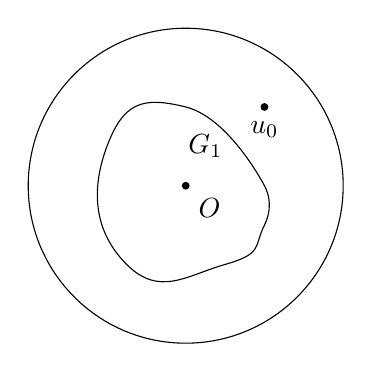
\begin{tikzpicture}
            \draw (0,0) circle (2);
            \draw [-] plot [smooth, tension=1] coordinates {(1,0) (0,1) (-1,0.5) (-0.75,-1) (0.5,-1) (1,-0.5) (1,0)};
            \node[fill,circle,inner sep=1pt,label=below right:$O$] at (0,0) {};
            \node[fill,circle,inner sep=1pt,label=below:$u_0$] at (1,1) {};
            \node at (0.25, 0.5) {$G_1$};
        \end{tikzpicture}
    };

    \node(c) at (16, 0) {
        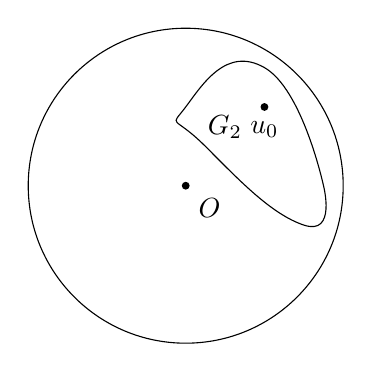
\begin{tikzpicture}
            \draw (0,0) circle (2);
            \draw [-] plot [smooth, tension=1] coordinates {(1.75,0) (1,1.5) (0,1) (0.25,0.5) (1.5,-0.5) (1.75,0)};
            \node[fill,circle,inner sep=1pt,label=below right:$O$] at (0,0) {};
            \node[fill,circle,inner sep=1pt,label=below:$u_0$] at (1,1) {};
            \node at (0.5, 0.75) {$G_2$};
        \end{tikzpicture}
    };

    \node(d) at (24, 0) {
        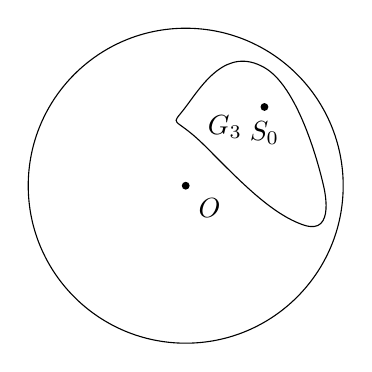
\begin{tikzpicture}
            \draw (0,0) circle (2);
            \draw [-] plot [smooth, tension=1] coordinates {(1.75,0) (1,1.5) (0,1) (0.25,0.5) (1.5,-0.5) (1.75,0)};
            \node[fill,circle,inner sep=1pt,label=below right:$O$] at (0,0) {};
            \node[fill,circle,inner sep=1pt,label=below:$S_0$] at (1,1) {};
            \node at (0.5, 0.75) {$G_3$};
        \end{tikzpicture}
    };

    \node(e) at (32, 0) {
        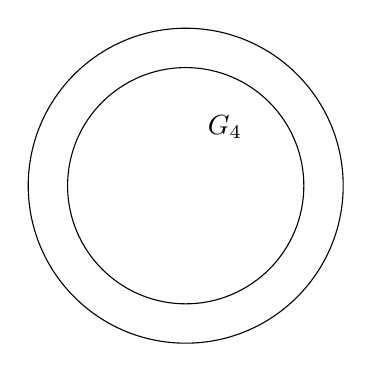
\begin{tikzpicture}
            \draw (0,0) circle (2);
            \draw (0,0) circle (1.5);
            \node at (0.5, 0.75) {$G_4$};
        \end{tikzpicture}
    };

    \draw[->] (a) -- (b);
    \node[above] at (4,0) {$f_{*}$};

    \draw[->] (b) -- (c);
    \node[above] at (12,0) {$\phi_{u_0}$};

    \draw[->] (c) -- (d);
    \node[above] at (20, 0) {$P(z) = \sqrt{z}$};

    \draw[->] (d) -- (e);
    \node[above] at (28, 0) {$q(z) = \dfrac{S_0}{\mid S_0 \mid} \phi_{u_0}$};
\end{tikzpicture}
\end{document}